\documentclass[serif,mathserif,final]{beamer}
\mode<presentation>{\usetheme{Lankton}}
\usepackage{amsmath,amsfonts,amssymb,pxfonts,eulervm,xspace}
\usepackage{graphicx}
\graphicspath{{./fig/}}
\usepackage[orientation=landscape,size=custom,width=40,height=30,scale=.6,debug]{beamerposter}

%-- Header and footer information ----------------------------------
\newcommand{\footleft}{https://github.com/hsavoy/cs267FinalProject}
\newcommand{\footright}{longva@berkeley.edu \quad frystacka@berkeley.edu}
\title{Parallel Empirical Variogram Calculation for Large Datasets}
\author{Andreas Borgen Longva \quad Heather Savoy}
\institute{University of California, Berkeley}
%-------------------------------------------------------------------


%-- Main Document --------------------------------------------------
\begin{document}
\begin{frame}{}
  \begin{columns}[t]

    %-- Column 1 ---------------------------------------------------
    \begin{column}{0.32\linewidth}

      %-- Block 1-1
      \begin{block}{Motivation}
   
	 \begin{itemize}
	 	\item Spatial heterogeneity in an aquifer significantly affect contaminant transport in groundwater
		\item A way is needed to incorporate the uncertainty about the aquifer in groundwater modeling (geostatistics!)
         
         \begin{figure}[htbp]
            \centering
            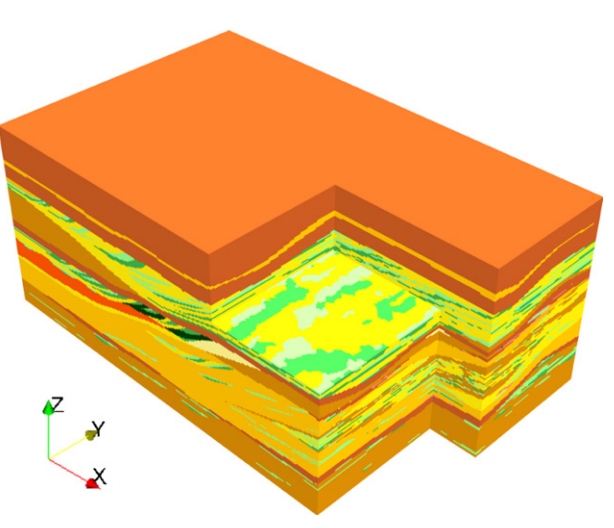
\includegraphics[height=5cm]{herten.png} % requires the graphicx package
            \caption{Large aquifer data set : $n=8.96\times 10^6$ \cite{Comunian2011a}}
            \label{fig:example}
         \end{figure}
         
         \item The data set above can be used to study realistic geologic patterns, but it is too big for serial geostatistical algorithms
          \end{itemize}
      \end{block}

      %-- Block 1-2
      \begin{block}{Geostatistics}
      Variograms describe how properties are correlated over space:
        \begin{equation*}
		\hat{\gamma}(h)=\frac{1}{2|N(h)|}\sum_{(i,j)\in N(h)} |z_i-z_j|^2
	\end{equation*}
	The algorithm is $O(n^2)$ and involves all-to-all communications
      \end{block}
  

    \end{column}%1

    %-- Column 2 ---------------------------------------------------
    \begin{column}{0.32\linewidth}

      %-- Block 2-1
      \begin{block}{Implementation}
      Communication Optimal \cite{Driscoll2013}
        \begin{itemize}
          \item 
        \end{itemize}
      Computation Optimal \cite{Koanantakool}
        \begin{itemize}
          \item 
        \end{itemize}
      \end{block}

    \end{column}%2

    %-- Column 3 ---------------------------------------------------
    \begin{column}{0.32\linewidth}

      %-- Block 3-1
      \begin{block}{Timing Results}
        Remember to put lots of figures on your poster... Nobody reads anymore!
      \end{block}

      %-- Block 3-2
      \begin{block}{Conclusion and Outlook}
        
      \end{block}

      %-- Block 3-3
      \begin{block}{References}
        \bibliographystyle{plain}
	{\footnotesize
	\bibliography{ref}}
      \end{block}

    \end{column}%3

  \end{columns}
\end{frame}
\end{document}
